\documentclass[spanish,11pt,a4paper]{article}
\usepackage[spanish]{babel}
\usepackage[utf8]{inputenc}
\usepackage[dvips]{graphicx}
\title{\Huge\bf{\underline{El número $\Pi$}}}
\author{\Large\bf Adriana Calvo\\ Alumna de la ULL\\}
\date{\today}

\begin{document}
\maketitle

\begin{abstract}
\begin{figure}[h]
\begin{center}
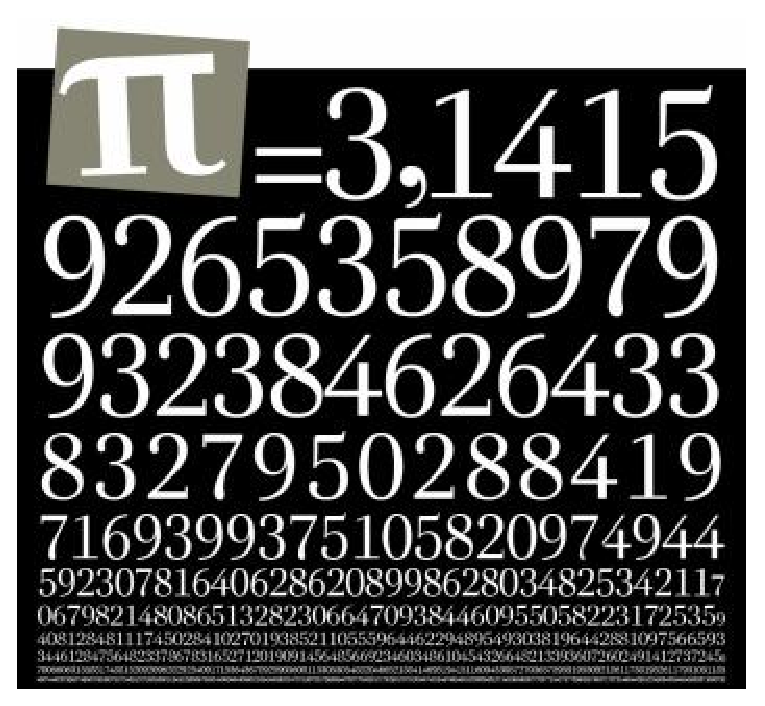
\includegraphics[width=0.75\textwidth]{images/foto1.eps}\end{center}
\caption{Aproximación}
\end{figure}

{\it\large El valor de $\Pi$ se ha obtenido con diversas aproximaciones a lo largo de la historia, siendo una de las constantes matemáticas que más aparece en las ecuaciones de la física, junto con el número $e$. Cabe destacar que el cociente entre la longitud de cualquier circunferencia y la de su diámetro no es constante en geometrías no euclídeas.}
\end{abstract} 

\section{Historia del cálculo de pi}
Nos encontramos con el número $\Pi$ cuando dividimos la longitud de una circunferencia entre su diámetro. Podemos hallar una aproximación con cualquier objeto redondo como, por ejemplo, un bote de conservas. Para llevar a cabo el experimento he buscado uno en mi despensa y lo he medido. He obtenido para la longitud de la circunferencia 26'7 cm, y para el diámetro 8'5 cm. 

Al dividir la longitud (26'7) entre el diámetro (8'5) se obtiene 3'141176... (que está muy cerca del valor teórico). Los objetos redondos (ruedas, recipientes...) fueron utilizados por el hombre desde muy antiguo. En algún momento debieron darse cuenta de que ese ''tres y un poc'' era fundamental para calcular las longitudes, áreas y volúmenes de los cuerpos redondos. 
Acontinuación veremos la historia del número Pi en distintas culturas.

\subsection{Antiguo egipto}

El valor aproximado de $\Pi$ en las antiguas culturas se remonta a la época del escriba egipcio Ahmes en el año 1800 a. C., descrito en el papiro Rhind,3 donde se emplea un valor aproximado de $\Pi$ afirmando que el área de un círculo es similar a la de un cuadrado cuyo lado es igual al diámetro del círculo disminuido en 1/9; es decir, igual a 8/9 del diámetro. 
Entre los ocho documentos matemáticos hallados de la antigua cultura egipcia, en dos se habla de círculos. Uno es el papiro Rhind y el otro es el papiro de Moscú. Sólo en el primero se habla del valor aproximado del número $\Pi$. El investigador Otto Neugebauer, en un anexo de su libro The Exact Sciences in Antiquity,4 describe un método inspirado en los problemas del papiro de Ahmes para averiguar el valor de $\Pi$, mediante la aproximación del área de un cuadrado de lado 8, a la de un círculo de diámetro 8.

\subsection{Mesopotamia}
Algunos matemáticos mesopotámicos empleaban, en el cálculo de segmentos, valores de $\Pi$ igual a 3, alcanzando en algunos casos valores más aproximados, como el de:

    $$\Pi \approx 3 + \frac{1}{8} = 3,125$$ 
\subsection{China} 
El cálculo de $\Pi$ fue una atracción para los matemáticos expertos de todas las culturas. Hacia 120, el astrónomo chino Zhang Heng (78-139) \cite{Wiki} fue uno de los primeros en usar la aproximación $\sqrt{10}$, que dedujo de la razón entre el volumen de un cubo y la respectiva esfera inscrita. Un siglo después, el astrónomo Wang Fang lo estimó en 142/45 (3,155555), aunque se desconoce el método empleado Pocos años después, hacia 263, el matemático Liu Hui fue el primero en sugerir que 3,14 era una buena aproximación, usando un polígono de 968 o 1926 lados. Posteriormente estimó $\Pi$ como 3,14159 empleando un polígono de 3.072 lados.8 9

A finales del siglo V, el matemático y astrónomo chino Zu Chongzhi \cite{Wiki} calculó el valor de $\Pi$ en 3,1415926, al que llamó «valor por defecto», y 3,1415927, «valor por exceso», y dio dos aproximaciones racionales de $\Pi$, 22/7 y 355/113, muy conocidas ambas,10 siendo la última aproximación tan buena y precisa que no fue igualada hasta más de nueve siglos después, en el siglo XV.
Acontinuación algunas aproximaciones históricas de valor de $\Pi$ \cite{Libro1}

\begin{tabular}{lcccc}
Año & Matemático & Cultura & Aproximación & Error\\
\hline
1900 a.C. & Papiro de Ahmes & Egipcia & 3,1605 & 6016 ppm\\
1600 a.C. & Tablilla de Susa & Babilónica & 3,125 & 5282 ppm\\
600 a.C. & La Biblia & Judía & 3,2143 & 4570 ppm\\
500 a.C. & Bandhayana & India & 3,09 & 16422 ppm

\end{tabular}

    
\section{Caracterízticas mátematicas}
Euclides fue el primero en demostrar que la relación entre una circunferencia y su diámetro es una cantidad constante.15 No obstante, existen diversas definiciones del número $\Pi$, pero las más común es:
\begin{itemize}

\item $\Pi$ es la relación entre la longitud de una circunferencia y su diámetro.

Por tanto, también $\Pi$ es:

\item El área de un círculo unitario (de radio unidad del plano euclídeo).
\item El menor número real x positivo tal que $\sin(x) = 0$.

También es posible definir analíticamente $\Pi$; dos definiciones son posibles:

\item La ecuación sobre los números complejos $e^{ix}+1=0$ admite una infinidad de soluciones reales positivas, la más pequeña de las cuales es precisamente $\Pi$ (véase identidad de Euler).
\item La ecuación diferencial $S''(x)+S(x)=0$ con las condiciones de contorno $S(0)=0, S'(0)=1$ para la que existe solución única, garantizada por el teorema de Picard-Lindelöf, es un función analítica (la función trigonométrica $\sin(x)$) cuya raíz positiva más pequeña es precisamente $\Pi$.
\end{itemize}



\begin{thebibliography}{3}
\bibitem{Wiki} Wikipedia
\bibitem {Libro1} Libro de historia de las matemáticas.
\bibitem {Libro2} Libro de juegos de lógica.
\end{thebibliography}

\footnote{$http://www.facultades.ull.es/Private/folder/centros
/matematicas/gradomat/informaciongeneral/mem_grado_
matematicas_marzo2010.pdf$}
\end{document}

